% Template for Cogsci submission with R Markdown

% Stuff changed from original Markdown PLOS Template
\documentclass[10pt, letterpaper]{article}

\usepackage{cogsci}
\usepackage{pslatex}
\usepackage{float}
\usepackage{caption}

% amsmath package, useful for mathematical formulas
\usepackage{amsmath}

% amssymb package, useful for mathematical symbols
\usepackage{amssymb}

% hyperref package, useful for hyperlinks
\usepackage{hyperref}

% graphicx package, useful for including eps and pdf graphics
% include graphics with the command \includegraphics
\usepackage{graphicx}

% Sweave(-like)
\usepackage{fancyvrb}
\DefineVerbatimEnvironment{Sinput}{Verbatim}{fontshape=sl}
\DefineVerbatimEnvironment{Soutput}{Verbatim}{}
\DefineVerbatimEnvironment{Scode}{Verbatim}{fontshape=sl}
\newenvironment{Schunk}{}{}
\DefineVerbatimEnvironment{Code}{Verbatim}{}
\DefineVerbatimEnvironment{CodeInput}{Verbatim}{fontshape=sl}
\DefineVerbatimEnvironment{CodeOutput}{Verbatim}{}
\newenvironment{CodeChunk}{}{}

% cite package, to clean up citations in the main text. Do not remove.
\usepackage{cite}

\usepackage{color}

% Use doublespacing - comment out for single spacing
%\usepackage{setspace}
%\doublespacing


% % Text layout
% \topmargin 0.0cm
% \oddsidemargin 0.5cm
% \evensidemargin 0.5cm
% \textwidth 16cm
% \textheight 21cm

\title{Children's understanding of simple polite markers}


\author{{\large \bf } \\ \texttt{} \\  \\}

\begin{document}

\maketitle

\begin{abstract}
Here we show that, with an improvement over the age of 2 to 4 years,
English-speaking preschool children understand implications of simple
polite markers: They understand that it is more polite and nicer (and
less rude and mean) to use polite markers such as ``please'' and ``can
you \textasciitilde{}'' when making requests, and that the use of these
polite markers indicates that the speaker is more socially likeable and
is more likely to gain compliance from their conversational partners.

\textbf{Keywords:}
Politeness, pragmatic development, online experiment
\end{abstract}

\section{Introduction}\label{introduction}

As adults, we use polite speech all the time.

Children produce polite speech early on.

Less work has looked at children's comprehension of polite speech.

For example, Nippold, Leonard, \& Anastopoulos (1982) looked at\ldots{}

In this current work, we sought to test what 2- to 4-year-old children
understand about polite speech. Specifically, we asked whether children
are sensitive to speakers' use of polite markers such as ``please'' and
``can you,'' and whether they: (1) reason about which speaker is being
more ``polite'' or ``rude'' (or ``nice'' or ``mean''); (2) reason about
social implications (e.g., play partner choice); and (3) show
improvement in their reasoning with increasing age.

Across three Experiments, we presented stories about speakers who
decided to speak politely (e.g., ``Please pour me more water'') or
impolitely (e.g., ``Pour me more water'') and asked child participants
to compare between the two speakers. In Experiment 1 and 2, we found
that 3- to 4-year-old children were able to reason that a speaker who
used polite markers was more polite and nicer than a speaker who did
not, and that the polite speaker is more socially likeable and is more
likely to gain what they want, given facial expression and prosodic
cues. In Experiment 3, we recruited two samples (one from a local
nursery school and the other from an online platform) and found that
children were able to reason correctly about polite speech even when the
supportive facial and prosodic cues were removed, and this reasoning
improves from 2 to 4 years of age.

\section{Experiment 1}\label{experiment-1}

In Experiment 1, we tested whether 3- to 4-year-old children were able
to understand implications of using simple polite markers, based on not
only linguistic cues of interest (whether the speaker says ``please,''
``can you''), but also extra cues that they might need (facial
expressions and prosodic cues). Thus, we asked children to compare
between speakers who used polite markers with a kind voice and facial
expression versus speakers who did not use polite markers and spoke with
a mean, angry voice and facial expression.

\subsection{Methods}\label{methods}

\subsubsection{Participants}\label{participants}

3-year-old (\(n=\) 20; 12 F, \(M_{age}\) = 3.61 years, \(SD_{age}\) =
0.22) and 4-year-old children (\(n=\) 18; 6 F, \(M_{age}\) = 4.38 years,
\(SD_{age}\) = 0.25) were recruited from a local preschool. An
additional 3 children were tested but excluded due to failure on the
practice questions (\(n=\) 2) or completion of fewer than half of the
test trials (\(n=\) 1).

\subsubsection{Stimuli and design}\label{stimuli-and-design}

We designed a picture book with twelve stories in which a protagonist is
approached by two speakers, one of whom makes a request by producing an
utterance with a polite marker (e.g., ``Please pour me more water''),
and the other produces an utterance without (``Pour me more water'').
There were three types of polite marker that could be used: ``please''
(as in ``Please pour me more water''), ``can you'' (``Can you pour me
more water''), and ``can you please'' (``Can you please pour me more
water'').

We designed six question types to ask participants following the
presentation of the stories: four \emph{speaker attribute} questions
(\emph{polite}: ``Which one was more polite?''; \emph{rude}: ``Which one
was more rude?''; \emph{nice}: ``Which one was nicer?''; \emph{mean}:
``Which one was meaner?'') and two \emph{social implication} questions
(\emph{play partner}: ``Which one would you rather play with?'';
\emph{compliance}: ``Which one will {[}get what they want{]}?''). Each
participant would be asked one of the four speaker attribute questions,
followed by one of the two social implication questions.

In Experiment 1, all utterances were produced live by the experimeter,
with appropriate proodic cues and facial expressions for each request:
thus, utterances with polite markers were produced by kind voice and
facial expression, whereas utterances lacking polite marker were
produced with angry voice and facial cues.

\subsubsection{Procedure}\label{procedure}

The experimenter presented to the child a storybook with a total of
thirteen stories about different characters. In the \emph{practice}
phase, the child heard a story with one clearly mean character
(\emph{Drew kicked Carol}) and one clearly nice character (\emph{Graham
gave Carol a gift}). After a reminder of what each character did, the
experimenter asked the participant: \emph{Which one was being meaner?}
and \emph{Which one was being nicer?} If the child answered the question
wrong the first time, the experimenter read the story one more time,
saying, ``Let's think about the story one more time.'' Only children who
correctly answered both questions in the first or second attempt were
included in the analyses.

In the \emph{test} phase, the child heard twelve stories, in each of
which they saw one speaker who decided to speak politely (\emph{Jean
wanted more water in her cup. Jean said to Fred, ``Please pour me more
water''}) and another speaker who spoke impolitely (\emph{Suzy also
wanted more water in her cup. Suzy said to Fred, ``Pour me more
water.''}). After a reminder about what each speaker said, the child was
asked a total of two questions. For the first question, the experimenter
asked one out of four possible questions for speaker attribute: ``Which
one was being more polite {[}more rude/nicer/meaner{]}?'' For the
second, social implication question, the experimenter either asked about
play partner (\emph{Which one would you rather play with?}) or
likelihood of compliance (e.g., \emph{Which one will Fred give water
to?}). The order of story types and question types was counterbalanced.

\subsection{Results and Discussion}\label{results-and-discussion}

\begin{CodeChunk}
\captionsetup{width=0.8\textwidth}\begin{figure*}[h]

{\centering 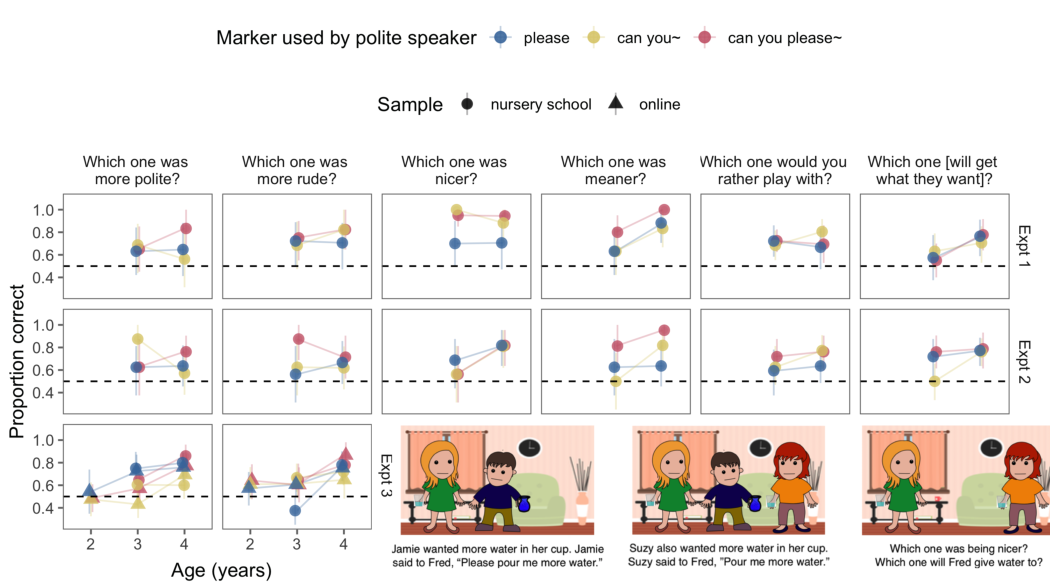
\includegraphics{figs/fig_results_placement-1} 

}

\caption[Bottom right]{Bottom right: Story example. Top, left: Results. Proportion of correct responses to questions comparing between a speaker who used a polite marker (where blue indicates "please", yellow "can you", and red "can you please") versus a speaker who did not. Data are binned into one-year age groups. Each row represents data from a different Experiment. Columns represent different questions asked. Dashed line represents chance level at 50\% (i.e., if participant were guessing at random).}\label{fig:fig_results_placement}
\end{figure*}
\end{CodeChunk}

We looked at the proportion of correct responses to various questions to
compare between a speaker who used a polite marker and spoke kindly,
versus a speaker who did not use a polite marker and spoke meanly
(Figure~\ref{fig:fig_results_placement}, first row). Both 3- and
4-year-olds overall gave correct answers when asked to compare between a
speaker who said ``Can you please\textasciitilde{}'' and a speaker who
did not (all \(t<\).05 except 3-year-olds not answering the
\emph{polite} questions correctly, see below), which suggested that
children at this age do pay attention to how the speakers make requests
and determine their attributes (``Because Jean said''please``, Jean was
nicer than Suzy'') and social implications of their actions (``Fred will
pour water in Jean's cup'').

For other markers, the performance varied depending on the age and type
of question asked. Both 3- and 4-year-olds overall seemed to struggle
with the \emph{polite} question (``Which one was more polite?''), though
4-year-olds did successfully answer that a speaker who said ``Can you
please\textasciitilde{}'' was more polite. 3-year-olds also struggled
with the \emph{compliance} question (``which one will {[}get what they
want{]}?''), whereas they accurately answered the \emph{play partner}
question (``Which one would you rather play with?''; all \(t<\).05),
suggesting that at 3 years children already become sensitive to some
social implications of speaking politely. Improvement over age was
clear, however, as 4-year-olds answered questions more accurately
overall for most of the question types.

A mixed-effects logistic regression predicting accuracy based on age,
question type and marker type\footnote{for Experiments 1 and 2, we use
  this model structure:
  \texttt{accuracy\ \textasciitilde{}\ age\ x\ question\ type\ x\ marker\ type\ +\ (1\ \textbar{}\ item)},
  where age is centered and scaled. All categorical variables were
  deviation coded, with specified contrasts of interest for the question
  type. Significance was calculated using the standard normal
  approximation to the \(t\) distribution ({\textbf{???}}).} confirmed
that there was an improvement with age (\(\beta\) = 0.2, \(p =\) 0.026),
and that children answered questions more accurately about a speaker who
used ``can you please'' compared to ``please'' (\(\beta\) = 0.28,
\(p =\) 0.038).

The regression model also confirmed that children seemed to find some
question types easier than others: Responses to \emph{nice} and
\emph{mean} questions were more accurate than to \emph{polite} and
\emph{rude} questions (\(\beta\) = 0.8, \(p =\) 0.002), whereas social
implication questions (\emph{play partner} and \emph{compliance}) were
overall more difficult compared to speaker attribute questions
(\emph{polite}, \emph{rude}, \emph{nice}, and \emph{mean}; \(\beta\) =
-0.33, \(p =\) 0.006).

In sum, in this first experiment, we saw preliminary evidence that
children pay attention to and understand some cues to politeness and are
able to use these cues to infer whether speakers are relatively polite,
rude, nice or mean, and whether speakers are good play partners and are
likely to gain what they wanted from their addressees. 4-year-olds
answered questions accurately more often compared to 3-year-olds, but
both age groups tended to be accurate when all the possible cuess were
used to signal that one speaker was polite (used ``can you
please\textasciitilde{}'', spoke with a kind tone and face) and the
other speaker wasn't (did not use a polite marker, spoke with an angry
tone and face).

However, one possible explanation for the finding in Experiment 1 is
that children are not using the linguistic polite markers (e.g.,
``please'') per se, and rather prosodic and facial cues that accompany
these markers. That is, children may have relied on the speaker's kind
voice and face rather than their use of ``please'' to evaluate their
niceness or likeability as a play partner. Similarly, greater accuracy
for some questions over others (e.g., ``nice'' \textgreater{}
``polite'') may have been due to greater association between some of the
words and prosodic and facial cues (e.g., a kind face may be seen to
signal niceness more than politeness), not due to greater understanding
for those words or concepts. Another potential concern is that the
experimenter was aware of the manipulations (i.e., they knew which
speaker was supposed to be ``polite'') and thus could have affected the
presentation of these speakers in ways that are not consistent across
all participants. In our next two experiments, we sought to address
these issue, and remove potentially confounding cues.

\section{Experiment 2}\label{experiment-2}

In Experiment 1, we saw initial evidence that children are able to use
some combinations of linguistic, prosodic, and facial cues to
politeness. In Experiment 2, we examined whether children are able to
make similar judgments using linguistic and prosodic cues only, without
facial expressions. For this, we used pre-recorded voiceovers to present
speaker utterances, so that (1) we could look at children's judgments
based on linguistic markers and prosodic cues only, and (2) we could
remove the role of potential bias of the experimenter in presentation of
these utterances.

\subsection{Methods}\label{methods-1}

\subsubsection{Participants}\label{participants-1}

3-year-old (\(n=\) 16; 8 F, \(M_{age}\) = 3.56 years, \(SD_{age}\) =
0.29) and 4-year-old children (\(n=\) 22; 13 F, \(M_{age}\) = 4.5 years,
\(SD_{age}\) = 0.32) were recruited from a local preschool. An
additional 5 children were tested but excluded due to failure on the
practice questions.

\subsubsection{Stimuli and design}\label{stimuli-and-design-1}

The design was identical to Experiment 1. Stimuli were the same as
Experiment 1 except two changes: (1) Instead of a picture book, we
presented the stories on a tablet; (2) the speakers' utterances were now
presented as recorded voiceovers. The voiceovers were recorded by native
English speakers, and contained prosodic cues that matched the
presence/absence of a polite marker (e.g., ``Please pour me more water''
was recorded with a kind voice and ``pour me more water'' with an angry
voice).

\subsubsection{Procedure}\label{procedure-1}

The procedure was identical to Experiment 1, except for the following
change: The participants now had to tap on a speaker on tablet in order
either to hear them speak, or to choose an answer to the questions
asked.

\subsection{Results and Discussion}\label{results-and-discussion-1}

Overall we saw similar patterns of results in Experiment 2 compared to 1
(Figure~\ref{fig:fig_results_placement}, second row).

Children made accurate judgments more often when the marker used was
``can you please'' compared to ``please'' (\(\beta\) = 0.39, \(p =\)
0.001)

There was an effect of age (\(\beta\) = 0.25, \(p =\) 0.002).

There was no main effect of question type, but there was an interaction
between age and question type such that performance for \emph{nice} and
\emph{mean} questions saw greater improvement with age than for
\emph{polite} and \emph{rude} questions (\(\beta\) = 0.57, \(p =\)
0.011).

In sum, across Experiments 1 and 2, we were able to confirm that, as
they get older, children get better in their use of politeness cues to
respond to questions about speaker attributes and social implications,
and that children make more accurate judgment to compare between
speakers based on their use of ``can you please'' compared to
``please.''

Next, we wanted to see whether children are able to evaluate speakers
based on linguistic markers only, without any other supporting cues such
as prosodic cues or facial expressions.

\section{Experiment 3}\label{experiment-3}

\subsection{Methods}\label{methods-2}

\subsubsection{Participants}\label{participants-2}

We recruited two samples of participants: one from the same local
nursery school as Experiments 1 and 2, and the other from Lookit
(\url{https://lookit.mit.edu/}), an online platform for child research
participation, in which parents and their children can participate
together. The nursery school sample consisted of 3-year-old (\(n=\) 24;
11 F, \(M_{age}\) = 3.65 years, \(SD_{age}\) = 0.26) and 4-year-old
children (\(n=\) 25; 13 F, \(M_{age}\) = 4.48 years, \(SD_{age}\) =
0.28). An additional 3 children were tested but excluded due to failure
on the practice questions.

The online sample consisted of 2-year-old (\(n=\) 23; 12 F, \(M_{age}\)
= 2.48 years, \(SD_{age}\) = 0.29), 3-year-old (\(n=\) 31; 15 F,
\(M_{age}\) = 3.59 years, \(SD_{age}\) = 0.27) and 4-year-old children
(\(n=\) 27; 12 F, \(M_{age}\) = 4.46 years, \(SD_{age}\) = 0.29). An
additional 32 children were tested but excluded due to failure on the
practice questions (\(n=\) 19) or completion of fewer than half of the
test trials (\(n=\) 13).

\subsubsection{Stimuli}\label{stimuli}

For the nursery school sample, stimuli were identical to Experiment 2
except that the voiceovers for all utterances had the same prosody: All
utterances ended with a rising intonation. For the online sample,
stimuli were identical to what the nusery school participants saw except
that the story narration (other than speaker utterances) were also
pre-recorded such that parents did not need to read the stories aloud
themselves.

\subsubsection{Procedure}\label{procedure-2}

For the nursery school sample, the procedure was identical to Experiment
2. For the online sample, the procedure was similar except that parents
and children participated together at home and there was no experimenter
present. Parents accessed the webpage for the study and gave their
consent for participation, and then read instructions to proceed through
the different stories, which specified with an emphasis to not help
their children answer the questions.

\subsection{Results and Discussion}\label{results-and-discussion-2}

With an additional 2-year-old group included in the online sample, the
improvement trend with age was clear
(Figure~\ref{fig:fig_results_placement}, third row, bottom left). A
mixed-effects logistic regression predicting accuracy based on age,
question type and marker type, controlling for sample\footnote{Model
  structure:
  \texttt{accuracy\ \textasciitilde{}\ sample\ +\ age\ x\ question\ type\ x\ marker\ type\ +\ (1\ \textbar{}\ item)}}
showed improvement with age in accurately responding to the questions,
which was consistent with the two previous experiments. Thus,

\section{General Discussion}\label{general-discussion}

\section{References}\label{references}

\setlength{\parindent}{-0.1in} \setlength{\leftskip}{0.125in} \noindent

\hypertarget{refs}{}
\hypertarget{ref-nippold1982}{}
Nippold, M. A., Leonard, L. B., \& Anastopoulos, A. (1982). Development
in the use and understanding of polite forms in children. \emph{Journal
of Speech, Language, and Hearing Research}, \emph{25}(2), 193--202.

\end{document}
